\begin{frame}{data challenge revisited}{insufficiency vs. representativeness}
		\hspace{-4mm}moderate improvements can be made to deal with insufficient data, but
		\visible<2->{
		\bigskip
		\question{is the amount of data really the main issue}}
		\pause
		\begin{itemize}
				\item	maybe not...
				\begin{itemize}
					\item a closer look at example music datasets for popular tasks
				\end{itemize}
		\end{itemize}
\end{frame}

\begin{frame}{data challenge revisited}{dataset example 1: chord detection}
    \vspace{-5mm}
    \begin{columns}
    \column{.8\linewidth}
        \begin{itemize}
            \item	Beatles dataset for chord detection
                \begin{itemize}
                    \item   chord progressions from Beatles albums (181 songs)
                    \item	chord vocabulary
                \end{itemize}
        \bigskip
        \item<2->	potential problems
            \begin{itemize}
                \item   stylistic homogeneity
                    \begin{itemize}
                        \item timbre and instrumentation, style, release dates, audio quality...
                    \end{itemize}
                \item	chord imbalance
                    \begin{itemize}
                        \item very skewed distribution, key dependence
                    \end{itemize}
            \end{itemize}
        \bigskip
        \item<3->[$\Rightarrow$] \textbf{may not generalize}
        \item<3->[$\Rightarrow$] \textbf{may only recognize most common chords}
        \end{itemize}
    \column{.2\linewidth}
        \begin{figure}%
            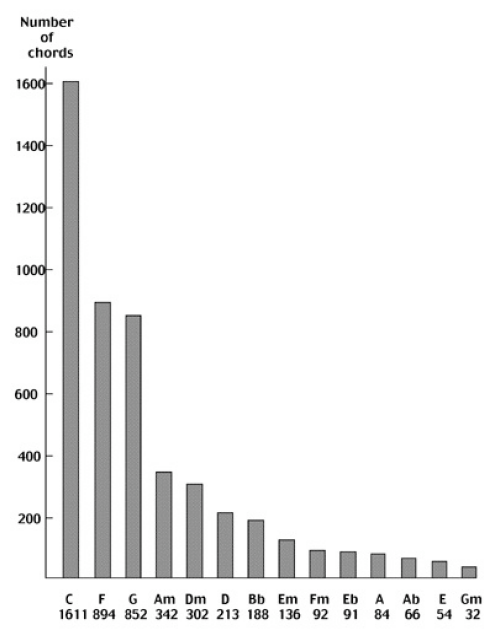
\includegraphics[width=\columnwidth]{beatles-chord-dist}%
        \end{figure}
    \end{columns}
\end{frame}

\begin{frame}{data challenge revisited}{dataset example 2: music genre classification}
    \vspace{-5mm}
    \begin{columns}
    \column{.8\linewidth}
    \begin{itemize}
        \item	GTZAN dataset for genre classification
            \begin{itemize}
                \item   10 classes
                \item   1000 \unit[30]{s} snippets
            \end{itemize}
        \bigskip
        \item<2->	problems with labeling
            \begin{itemize}
                \item   what are the 10 most relevant music genres, why 10?
                \item	how are genres categorized? examples:
                    \begin{itemize}
                        \item baroque, christmas songs, fugue, indian art music, symphony, fusion
                    \end{itemize}
                \item  single-label vs.\ multi-label
            \end{itemize}
        \bigskip
        \item<3->[$\Rightarrow$] \textbf{mismatch between dataset labels and 'real' task}
    \end{itemize}
    \column{.2\linewidth}
    \begin{itemize}
        \item[] \textit{Disco}
		\item[] \textit{Country}
		\item[] \textit{Hip Hop}
		\item[] \textit{Rock}
        \item[] \textit{Blues}
        \item[] \textit{Reggae}
        \item[] \textit{Pop}
        \item[] \textit{Metal}
        \item[] \textit{Classical}
        \item[] \textit{Jazz}
    \end{itemize}
    \end{columns}
\end{frame}

\begin{frame}{data challenge revisited}{dataset example 3: source separation}
    \vspace{-5mm}
    \begin{columns}
    \column{.8\linewidth}
    \begin{itemize}
        \item	MUSDB dataset for source separation
            \begin{itemize}
                \item   150 songs
                \item   4 stems: vocals, drums, bass, other
            \end{itemize}
        \bigskip
        \item<2->	problems
            \begin{itemize}
                \item   stem selection does not reflect many real world scenarios
                \item   dataset size cannot reflect a diverse set of popular music
            \end{itemize}
        \bigskip
        \item<3->[$\Rightarrow$] \textbf{mismatch between dataset and 'real' task}
    \end{itemize}
    \column{.2\linewidth}
    \end{columns}
\end{frame}

\begin{frame}{data challenge revisited}{dataset examples: summary}
		\begin{itemize}
			\item 	false homogeneity/\textbf{non-representativeness impacts generalization}
				\begin{itemize}
					\item system cannot learn what is hasn't seen or what seems irrelevant
				\end{itemize}
			\bigskip
			\item		imbalance can lead to \textbf{unwanted bias} 
				\begin{itemize}
					\item 	\textit{training}: system wrongly favors certain categories
					\item		\textit{testing}: results may imply good performance yet cannot be generalized
				\end{itemize}
			\bigskip
			\item		mismatch between dataset labels and real task may \textbf{feign good performance}
				\begin{itemize}
					\item 	misleading results
					\item		architectural bias
				\end{itemize}
		\end{itemize}
		%\begin{itemize}
			%\item 	systems might not generalize
			%\item		there is no way to judge as the evaluation is done on data with similar characteristics
				%\begin{itemize}
					%\item results may imply good performance yet cannot be generalized
				%\end{itemize}
			%\item		annotation choices and limitations might impact architectural decisions
		%\end{itemize}
\end{frame}